\documentclass[11pt]{article}

\usepackage[utf8]{inputenc}
\usepackage[T1]{fontenc}
\usepackage[default]{raleway}
\usepackage[english]{babel}
\usepackage[dvipsnames]{xcolor}
\usepackage[marginal, norule, perpage]{footmisc}
\usepackage{microtype}
\usepackage{graphicx}

\renewcommand{\thefootnote}{\Roman{footnote}}

\usepackage{hyperref}
\hypersetup{
  colorlinks=true,
  linkcolor=MidnightBlue,
  urlcolor=MidnightBlue
}

\title{
  \textbf{Project Hero}\\
  \large{Feasibility Study}
  \linebreak
  \linebreak
  \small{\texttt{01001000\\01000101\\01010010\\01001111}}
}

\author{
  \begin{tabular}{rl}
    \textbf{Team:}
    & \textsc{Djordjevic} Filip\\
    & \textsc{Reichl} Markus \small{\textit{(Project Manager)}}\\
    & \textsc{Tekin} Abdurrahim\\
    & \textsc{Wellner} Florian\\
    \\
    \textbf{Supervision:}
    & \textsc{Dolezal} Dominik
  \end{tabular}
}

\begin{document}
\begin{titlepage}
  \clearpage
  \maketitle
  \thispagestyle{empty}
  
  \begin{abstract}
    \begin{flushleft}
      Project Hero is a \textbf{bullethell roguelike multiplayer RPG} providing a very unique storytelling and gameplay experience.
      
      Its main goal is to create a solid base for a video game ready for further development. The core should be highly abstract, stable and easy to extend.
      \linebreak
      \linebreak
      This document goes into detail with the projects technical feasibility and reviews different approaches resulting into a clear conclusion and the best way to go.
     \end{flushleft}
  \end{abstract}
\end{titlepage}

\tableofcontents

\newpage

\section{Introduction}
Project Hero is a \textbf{
  bullethell
  \footnote{A video game sub-genre where the screen is usually covered in bullets.}
  roguelike
  \footnote{A video game sub-genre which, based on the \href{http://roguebasin.com/roguelike-definition}{Roguebasin Interpretation}, is defined by 
    \begin{itemize}
      \item \textbf{Permanent Failure:} The player is encouraged to take responsibility for the risks he takes.
      \item \textbf{Procedural Environments:} Most of the game world is generated and provides complexity in resources and other elements of the game.
      \item \textbf{Resources:} The player can manage a limited amount of resources.
    \end{itemize}
    The \href{http://roguebasin.com/roguelike-definition}{Roguebasin}, \href{http://roguebasin.com/index.php?title=Berlin_Interpretation}{Berlin} and \href{http://roguetemple.com/roguelike-definition}{Roguetemple} Interpretation may give a more detailed explanation on this subject.
  }
  multiplayer
  \footnote{A multiplayer game allows but does not require clients to play together. The Hero Project is not meant to be played online only!}
  RPG\footnote{A roleplay game is a game in which the player assumes the roles of characters in a fictional setting and takes responsibility for his acting either through literal acting.}
} providing a very unique storytelling and gameplay experience.

It is highly inspired by previous titles in the roguelike and roleplay game genres, the most noteworthy being \href{https://realmofthemadgod.com}{Realm of the Mad God}, \href{http://www.devolverdigital.com/games/view/titan-souls}{Titan Souls} and \href{http://dodgeroll.com/gungeon/}{Enter the Gungeon}.

While all mentioned games are using a topdown pixelart setting, the Hero Project is drawn in a very unique combination of high and low resolutions.

\newpage

\section{Project Goals}
The main goal of Project Hero is to create a solid base for a video game ready for further development.
This base includes all elements listed in the \textit{Functional} and \textit{Technical Requirements} sections found in the \textit{Requirement Specification} document.

\subsection{Targets}
Before development can start the aim of the project has to be as clear as possible. Therefore the following targets and non-targets have been declared.
\paragraph{Targets}
\subparagraph{A core game} A prototype ready for further development including all Functional and Technical Requirements. Date of of submission is set on 17th of January 2017.
\subparagraph{A prototype for presentation} A simple setup including a player, an enemy and items including effects to declare an attack.

\paragraph{Non Targets}
\subparagraph{A full game} The core game is not meant to provide a full game including graphics, gameplay and multiplayer. This goal is not reachable in time and may not be in budget.
\subparagraph{A demo version} The core game should demonstrate how the game works and how it can be extended. Not how the game will look like in production,

\newpage

\section{Technical Feasibility}
With a video game being an enormous software project this study is mostly technical which requires the reader to have at least basic knowledge about video games and software development.
Technical terms will still be explained as footnotes at the bottom of each page.

\subsection{Team}
Because the majority of the product will be developed by a rather small team each members technical experience and skill has a huge influence on the projects schedule and quality.
The Hero Projects core as a school project is developed by a static team of 4 members and 1 professor listed below.
\paragraph{\textsc{Djordjevic} Filip} ~\\
\begin{tabular}{ll}
\texttt{Roles} & Sound Designer\\
\texttt{Areas of expertise} & Music and Sound Design
\end{tabular}
\paragraph{\textsc{Reichl} Markus} ~\\
\begin{tabular}{ll}
\texttt{Roles} & Project Manager \textit{\small{(Product Owner)}}\\
\texttt{Areas of expertise} & Concept Art and System Architecture
\end{tabular}
\paragraph{\textsc{Tekin} Abdurrahim} ~\\
\begin{tabular}{ll}
\texttt{Roles} & Artist\\
\texttt{Areas of expertise} & Art and Design
\end{tabular}
\paragraph{\textsc{Wellner} Florian} ~\\
\begin{tabular}{ll}
\texttt{Roles} & Software Developer\\
\texttt{Areas of expertise} & Software Development
\end{tabular}
\paragraph{\textsc{Dolezal} Dominik} ~\\
\begin{tabular}{ll}
\texttt{Roles} & Professor \textit{\small{(Supervisor)}}\\
\texttt{Areas of expertise} & Software Development
\end{tabular}
\\
\\
\\
While providing a wide variety of skills the majority of the team is also well attuned. Everyone has at least some experience with video games but only a few have already worked on one.

\subsection{Requirement Analysis}
The following section analyses all Functional and Technical requirements found in the Requirements Specification document and gives some short information about the teams thoughts on their technical feasibility.

\subsubsection{Functional Requirements}
\paragraph{Artificial Intelligence}~\\
AIs are basically characters controlled by the game, which means that an AI differs from a character only by his controlling unit.
\paragraph{Character}~\\
A character, according to the Requirements Specification document, defines an entity controlled by the player.
It should be able to move, take actions and carry an inventory. The first two depend directly on the users input, which is hard to keep platform independent assuming that the game is not using another engine.
Implementing a levelling system for the player which interacts with a characters attributes should not be a problem.
\paragraph{Effects}~\\
In order to keep the core clean while adding lots of new features to the game effects have to be abstract and highly encapsulated. They should not depend on the identity of their owning entity and therefore work out of the box.
A decoupling pattern called the Component Pattern can be used to manage multiple effects and keep the game extendable. Most popular engines also rely on this pattern.
\paragraph{Items}~\\
In order to store items for multiple players at least some kind of a database is required. There are multiple solutions for this problem, lots of game engines even bring their own database implementations.
Items also have to be store- and even equipable by the player which makes them great candidates to hold effects the player can activate. Items should only usable by the player because they only interact through their effects which also covers the requirement \textit{Item Interaction}. 
This is possible because all other entities use effects as components directly.
\paragraph{Attributes}~\\
Attributes are simple values and can easily be interacted with.
They should also be treated like components and not be restricted to characters only.

\subsubsection{Technical Requirements}
\paragraph{Cross-Platform}~\\
Cross-Platform is hard to guarantee while not using an engine which is designed for multiple devices. Most programming languages nowadays can be used on any popular operating systems which at least fits the requirements.
Using an engine would allow the game to be ported to more platforms including consoles, smartphones and tablets.
\paragraph{Extendable}~\\
In order to keep the core extendable abstraction and decoupling are really important. All parts of the game have to work independently including later extensions.
\paragraph{Multiplayer Ready}~\\
Assuming a server while developing the core is not as easy as it seems but possible when considered from the start.
Here too an engine can help and improve the project lot.

\subsubsection{Conclusion}
The development process is quite intense and might not fit the schedule when every part of the game is hard coded. The team suggests using a framework which already provides essential components.
Possible candidates are engines like Gamemaker and \hyperref[subsubsec:unity]{Unity} or frameworks like \hyperref[subsubsec:monogame]{Monogame} or \hyperref[subsubsec:vulkan]{Vulkan}.

\newpage

\subsection{Engines and Frameworks}
Because of the volume of this project the team highly recommends using an engine which already provides key elements and can be easily extended.
After comparing lots of possible options the team decided on 3 major possibilities.

\subsubsection{Monogame}\label{subsubsec:monogame}
Monogame is an open-source framework based on Microsofts XNA-4\footnote{XNA Is Not Acronymed is a video game framework developed by Microsoft}. It provides cross-platform support and is optimised for 2D.
Popular games using Monogame include the indie game \href{http://store.steampowered.com/app/224760/}{FEZ}.

It allows but also requires the developer to write critical game code and is very lightweight.
\subsubsection{Unity}\label{subsubsec:unity}
Unity is a huge game engine and built for 3D games while also providing 2D support. It comes with a lot of features and a solid framework for both newbies and professional game developers.
Lots of popular games were developed in Unity recently including \href{http://www.oriblindforest.com}{Ori And The Blind Forest}, \href{https://playrust.com}{Rust} and one game also found in the Requirement Specification document \href{http://dodgeroll.com/gungeon/}{Enter the Gungeon}.
\subsubsection{Vulkan}\label{subsubsec:vulkan}
Vulkan is the next level of OpenGL released in 2016. Using Vulkan basically means working from scratch. It allows the user to work very close to the computers hardware and offers a lot of possibilities not found in OpenGL.
\newpage
\subsubsection{Comparison}
To compare these options the following table rates all features relevant for the project from a minimum of 1 to a maximum of 3.
\bigskip
\\
\begin{tabular}{l|l|l|l}
 & Monogame & Unity & Vulkan\\
 \hline
 Features 	& 2 & 3 & 1\\
 Documentation 	& 1 & 3 & 1\\
 Performance 	& 2 & 2 & 1\\
 Cross-Platform & 3 & 3 & 0\\
 Popularity 	& 1 & 3 & 1\\
 \hline
 & 9 & 14 & 4
\end{tabular}
\bigskip
\\
Looking at this short comparison it seems rather clear which framework is the one to choose.

\subsubsection{Conclusion}
Comparing all these engines and frameworks the team got really excited looking at the games running on Unity and its amazing features which would otherwise be really hard to implement. 
While Monogame and Vulkan give the developer a lot of freedom, Unity gives a whole swiss army knife. Looking at the teams schedule and the features the project needs Unity seems to be a great option and maybe the only option.

\newpage

\section{Economic Feasibility}
Although the core game itself is not sold to any user base the team did some research and gathered information about the market.
Right now there are many unknown and few popular bullethell roguelikes available including the four mentioned in the previous documents.

\subsection{Market Research}
A comparison of those games, their players and economics, can be found below. All information was gathered on the 26th September of 2016.

\paragraph{Realm of the Mad God}~\\
\begin{center}
 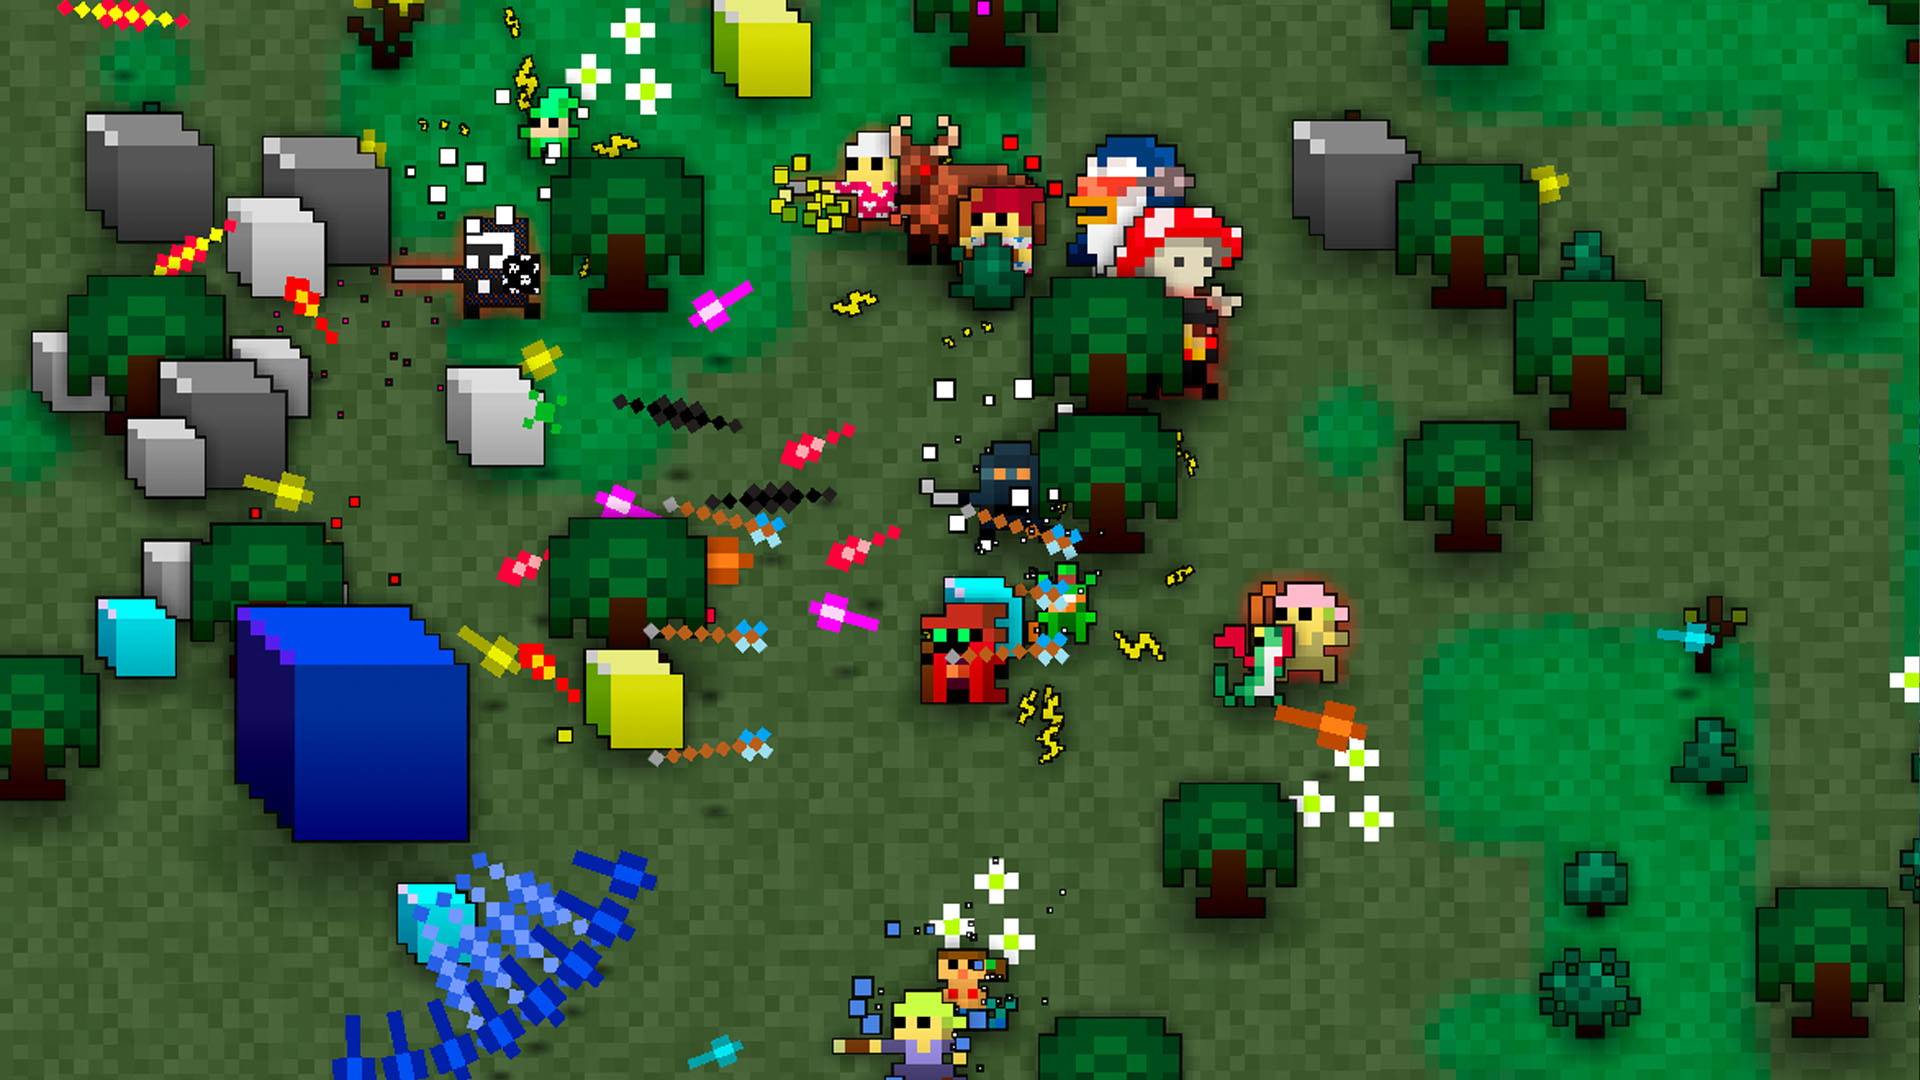
\includegraphics[width=\textwidth]{./rotmg.jpg}
\end{center}
Realm of the Mad God, or ROTMG for short, is a bullethell MMORPG\footnote{A massively multiplayer online role-playing game is a story-driven online video game in which a player interacts with a large number of other players.} currently played by 1.7 billion accounts.
It is free to play and makes profit from in game transactions which brought in 1.36 billion Euros in total since 2011.\\
While the game still has a high user base a lot of players actually wish for a better game.

\paragraph{Titan Souls}~\\
\begin{center}
 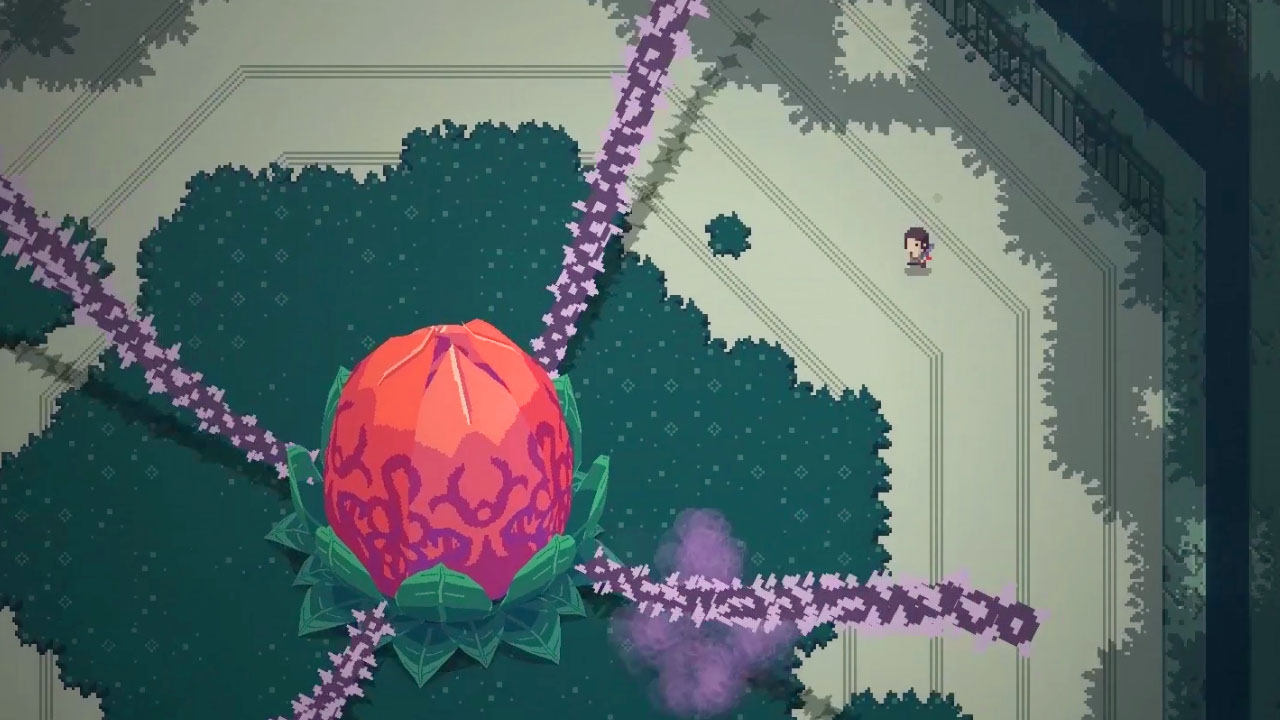
\includegraphics[width=\textwidth]{./titan.jpg}
\end{center}
Titan Souls is a roguelike RPG released in 2015. Since then it gathered 170 thousand players and acquired 1.65 billion Euros in total. It is available on steam for 14.99 Euros at the moment.
\bigskip

It uses a clear pixelart style and has basically no interface which improves gameplay a lot and makes a great game.

\newpage

\paragraph{Dungeon Souls}~\\
\begin{center}
 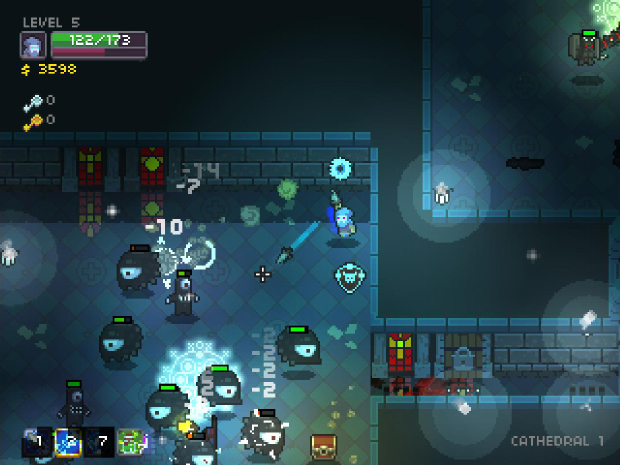
\includegraphics[width=\textwidth]{./dungeon.jpg}
\end{center}
Dungeon Souls is also a bullethell roguelike RPG released in 2015 and counts about 35 thousand players. It was developed by a indie studio and is now available on steam for 12.99 Euros which is quite a lot for this genre. 
The game gathered 300 thousand Euros since its release.

\newpage

\paragraph{Enter the Gungeon}~\\
\begin{center}
 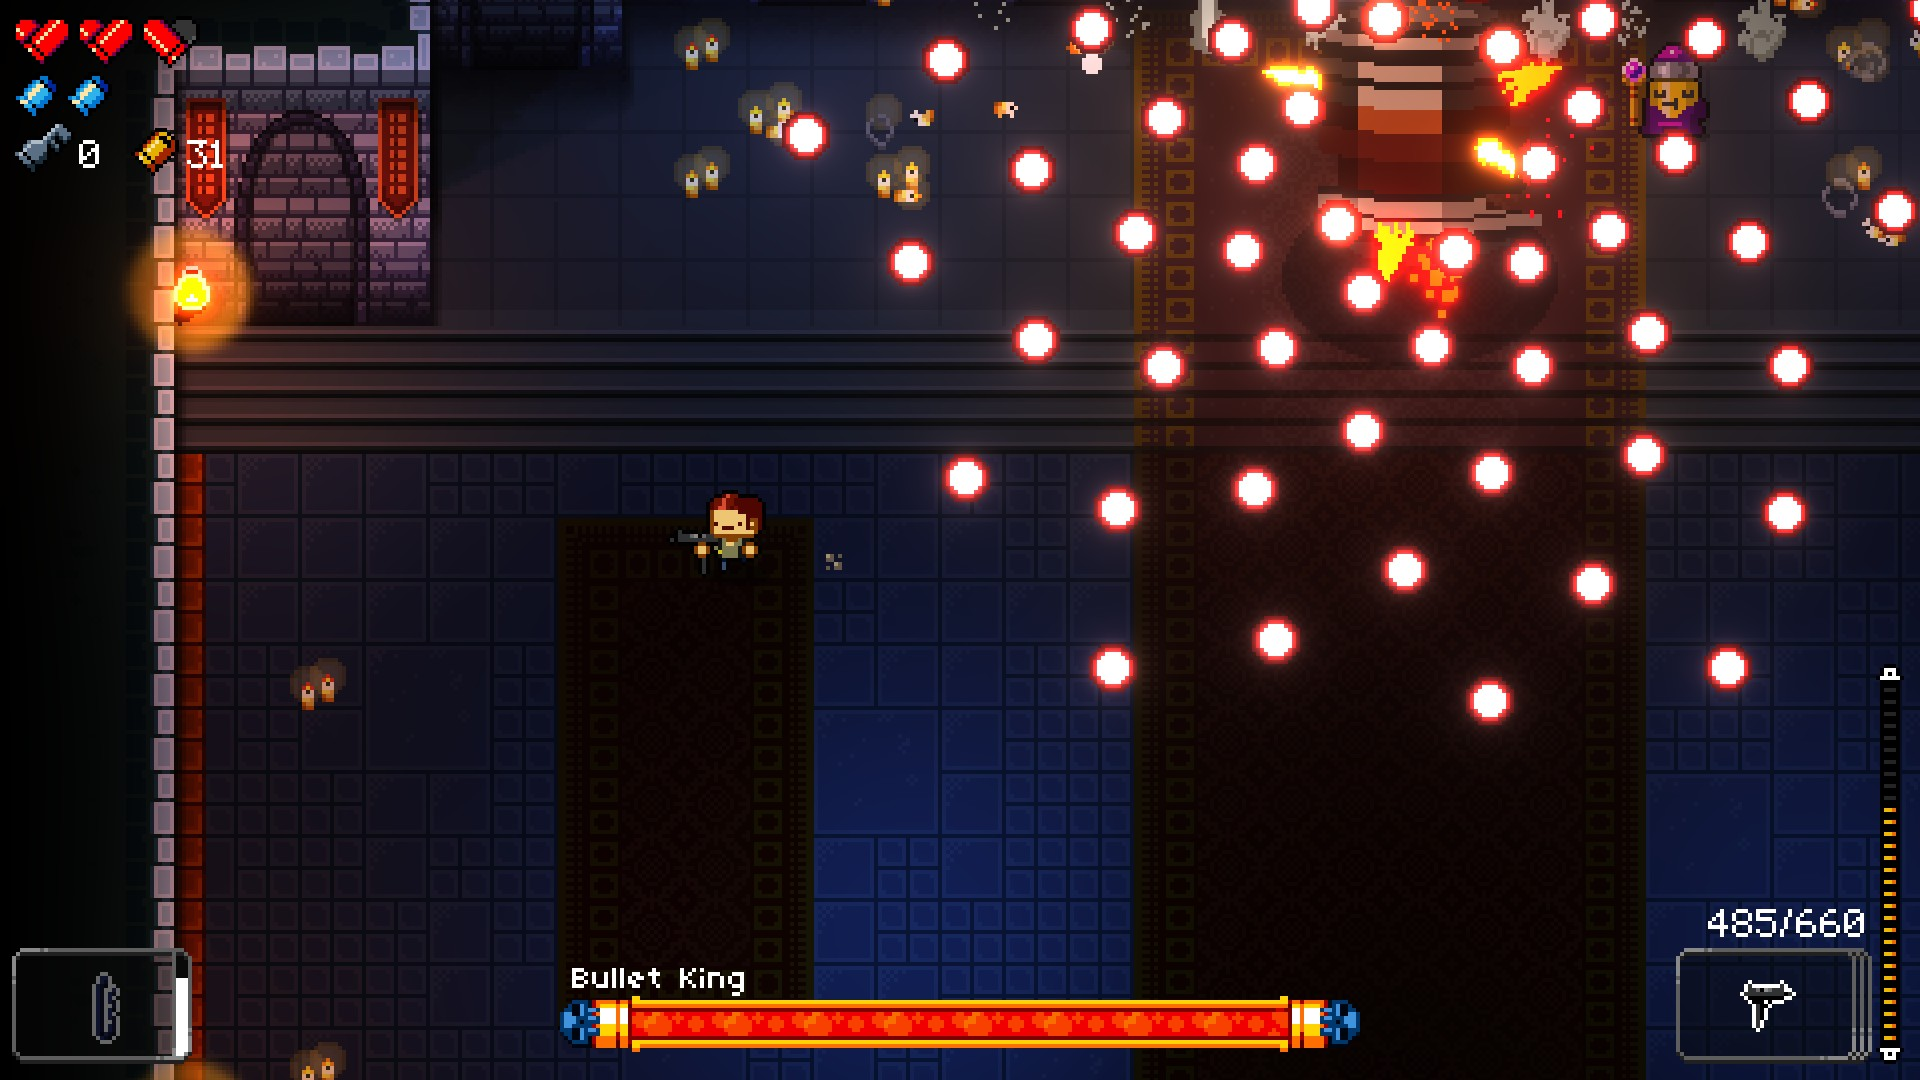
\includegraphics[width=\textwidth]{./gungeon.jpg}
\end{center}
Another bullethell roguelike RPG released in 2016 with a great art style and a huge user base of 414 thousand players which is quite a lot for an indie game. 
It is now sold for 14.99 Euros and gathered 4.095 billion Euros since its release.

\subsubsection{Conclusion}
The information gathered while researching for these games shows lots of possibilities but also sets high quality standards. 
There are many small indie developers in this genre but only few who rise to the top mostly because of their creativity or storytelling.

\newpage

\section{Schedule Feasibility}
Time is a very important factor in this project because it can become very consuming and may even take too long to be completed.
Due to the size of the team a single member can influence the schedule a lot.
\\
\\
Important milestones are the \textbf{prototype deadline} and the \textbf{project approval} on the 17th December of 2017 which gives the team a hundred days, excluding sun- and holidays, to provide the required specifications.

Although a hundred days would be quite enough while working 40 hours per week the team only has a regular work-time of 4 hours a week what leads to 60 hours per person which definitely is not enough to complete the project without a framework.

\section{Conclusion}
All features required by the previous document are viable and can be completed in time even though the development process will might become very intense.
An engine would help a lot, even more when the core game is finished and has to be extended. The team suggests using Unity for this purpose due to its large amount of features and solid base.

This said Project Hero is considered ready to start.

\end{document}
